\section{Basic Idea}

\noindent
The goal of a particle physics detector is to measure the 4-momenta of all particles produced in a collision and to identify their types.  As we discussed in the section on tracking, the 4-momenta of charged particles, such as electrons, pions, etc... whose $\left | \eta  \right |$ is not too large (usually less than about 2) can be measured by the tracker. However, we need another way to measure electrically neutral particles or ones at large. However, we need another way to measure electrically neutral particles or ones at large $\left | \eta  \right |$.

\;
\noindent
You may have already encountered the word ``calorimeter'' in your high school physics.  In thermodynamics, the temperature of a known (hot) object may be measured by immersing it in a bath and measuring the temperature rise of the bath.  The heat energy of the unknown object becomes that of a known object, allowing measurement. In a HEP calorimeter, the goal is to turn the kinetic energy of the particle into another type of energy that is more easily measured. In the process, the particle is altered so that it no longer reflects its initial properties (especially the momentum, but sometimes the type is changed) and no further useful measurements can be made.  Calorimeters should therefore be outside of the non-destructive detectors.

\;
\noindent
Remember our goal is to identify the 4-momentum and identify the type of all particles produced in the collisions. In a calorimeter, as we will discuss later, we can often use the shape of the energy deposit to tell if the particle is  either an electron or a photon (on the one hand) or a hadron. The calorimeter is segmented so the azimuthal ($\phi$) and polar angle ($\theta$) can be estimated, assuming the particle was produced at the center of the detector, by drawing a line from the production point to the impact point on the calorimeter face. If we assume the particle$'$s mass is small compared to its momentum (massless approximation), the particle$'$s momentum can be estimated as:

\begin{equation}\hspace{34 mm}p = E(l,cos(\theta ),cos(\phi ),cos(\theta ),sin(\phi ),sin(\theta ))\end{equation}

\;
\;

\section{Showers}

\noindent
In a particle physics calorimeter, we try to first change the neutral particles (photons, neutrons, K-longs) into charged particles. Then, we change single high energy charged particle into a very large number of low energy charged particles in such a way that the number we create is proportional to the kinetic energy of the initial high energy particle. The low energy charged particles travel through matter, interacting with the electrons in the material, transferring their kinetic energy to them, until all the initial kinetic energy is transferred to the material. That material then needs to make some kind of signal that can be detected. You can see a schematic of this process in figure ~\ref{fig:cal1}. An initial particle comes in, somehow interacting with the material of the calorimeter, and is changed gradually into a large number of low energy particles, that ``range out'' in the material. This process is called ``showering''.

\;
\;

\begin{figure}[h]
\centering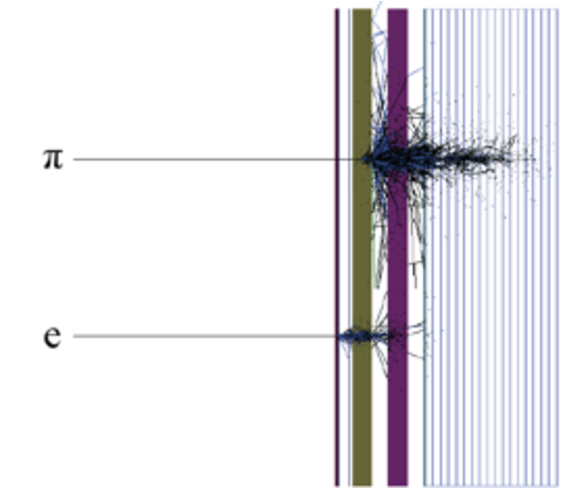
\includegraphics[scale=1.0]{./calorimetry/Pictures/fig1.pdf}
\caption{Schematic of a typical calorimeter. The front part is the ``Electromagnetic'' calorimeter and should contain the showers resulting from electrons and photons. The back of the calorimeter is the ``hadronic'' part, and should contain the showers resulting from particles containing quarks (mesons, baryons, etc).}
\label{fig:cal1}
\end{figure}

\;

\noindent
What are the processes that cause the creation of the secondary particles? That depends on whether the initial high energy particle was an ``EM'' particle (an electron or a photon) or a ``HAD'' particle (mesons, baryons).

\section{Electromagnetic Showers}

\noindent
An electromagnetic shower results when an electron or photon enters a thick piece of material with a large atomic number (Z). There are two main processes that occur:

\section{Bremsstrahlung}

\noindent
Bremsstrahlung is German for ``braking radiation'', and is a process that occurs for electrons. As you may have learned in your high school physics course, when a charged particle accelerates, it radiates electromagnetic radiation (photons, the particle of light). What would cause an electron to accelerate? An electron is a charged particle. A nucleus is also charged. For nuclei, such as lead or iron, that charge can be large. If an electron passes close enough to a nucleus, the electric force between the two particles causes the electron to accelerate (because the nucleus is much heavier than the electron, and is bound in the lattice of the solid, it does not move). Thus, in the presence of the nucleus, a high energy electron becomes a lower energy electron and a gamma ray (high energy photons). This can be draw as shown in figure ~\ref{fig:cal2}


\;
\;

\begin{figure}[h]
\centering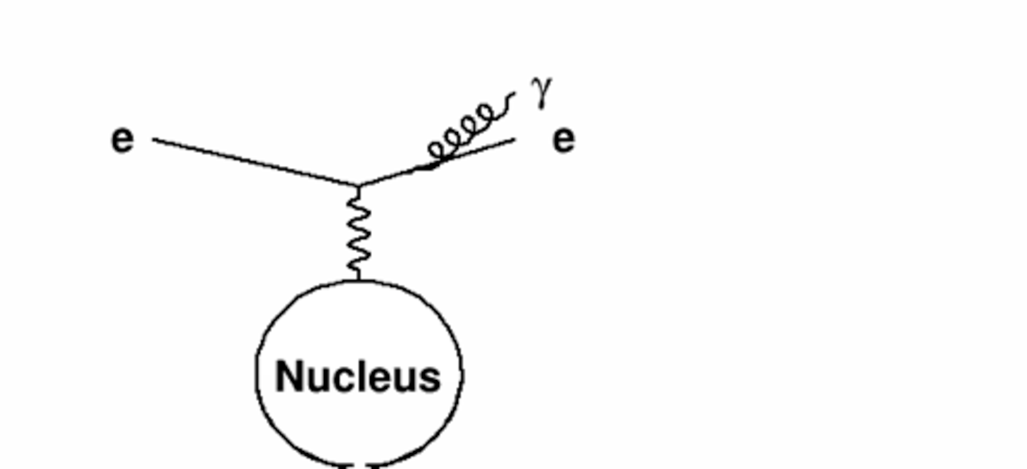
\includegraphics[scale=0.7]{./calorimetry/Pictures/fig2.pdf}
\caption{An electron radiates off a gamma ray in the presence of a nucleus.}
\label{fig:cal2}
\end{figure}

\;

\section{Pair Production}

\noindent
A similar process allows a high energy photon to become an electron-positron pair.  The energy of the photon must be at least twice the electron mass in order for this to not violate conservation of energy.  The Feynman diagram is shown in figure \ref{fig:cal3}.


\;
\;

\begin{figure}[h]
\centering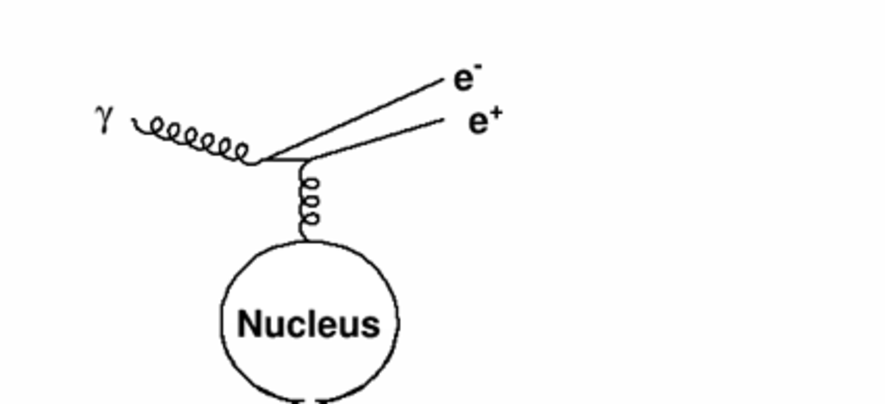
\includegraphics[scale=0.7]{./calorimetry/Pictures/fig3.pdf}
\caption{A high energy photon in the presence of a nucleus turns into an electron-positron pair}
\label{fig:cal3}
\end{figure}

\;

\section{Hadronic Showers}

\noindent
Electrons interact with the nucleus by producing electromagnetic interaction because of the electromagnetic force. Hadrons, however, can interact with nuclei via the strong force. This can cause a wide variety of processes to occur, often involving the break up of the nucleus. It takes more material to initiate a hadronic shower, as the hadron must pass closer to the nucleus, as the strong force is short range. A diagram of the resulting shower is shown in figure ~\ref{fig:cal4}

\;
\;

\begin{figure}[h]
\centering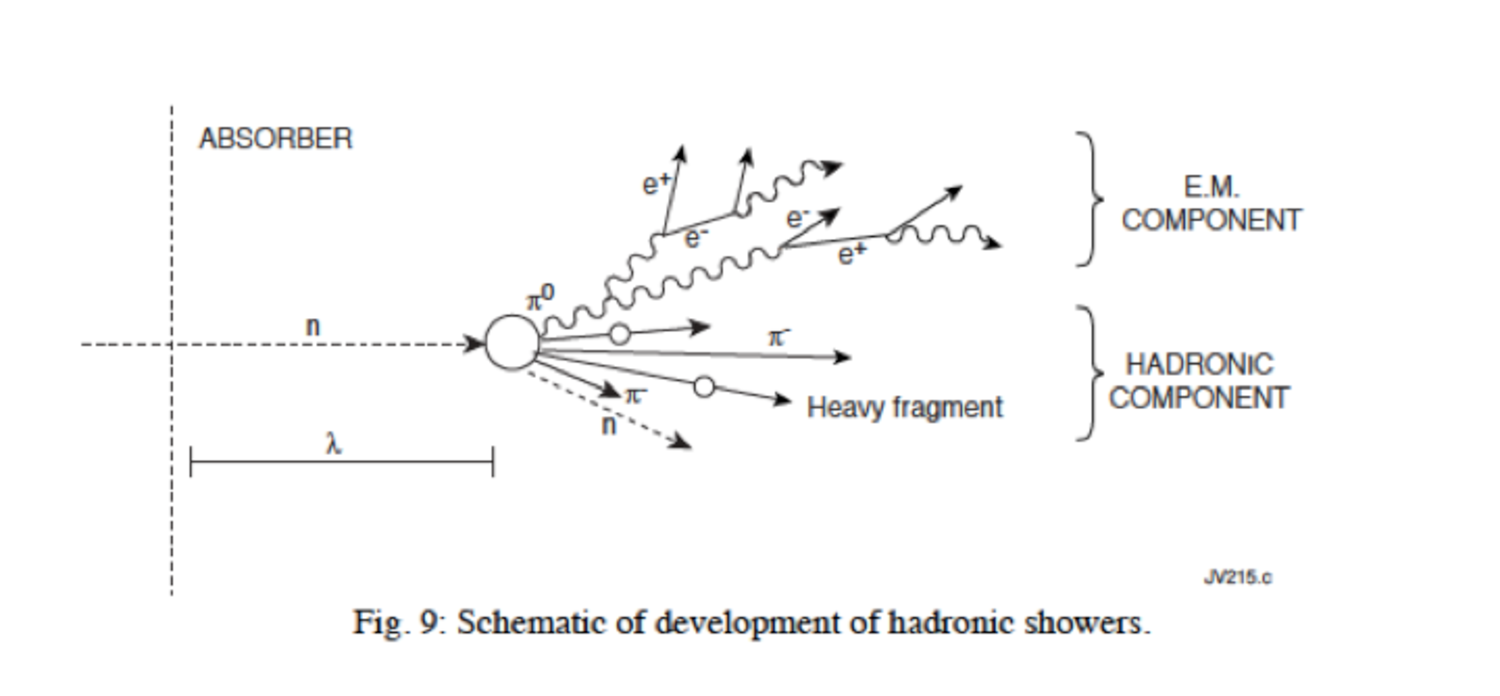
\includegraphics[scale=0.5]{./calorimetry/Pictures/fig4.pdf}
\caption{A figure showing a hadronic shower}
\label{fig:cal4}
\end{figure}

\;

\section{Detection}

\noindent
How do we measure the energy gained by the material? For many calorimeters, it is through the process of scintillation. Now, most high Z materials (think lead or uranium) do not scintillator, and are anyway opaque to light. So a calorimeter is often made of layers of the ``passive'' (high Z) material and the ``active'' (light producing) material, often plastic scintillator. A calorimeter that is like a smith island cake and has many layers is called a ``sampling'' calorimeter. The light produced by the scintillator is measuring using a photomultiplier tube or other light sensitive device (figure ~\ref{fig:cal5}).


\;
\;

\begin{figure}[h]
\centering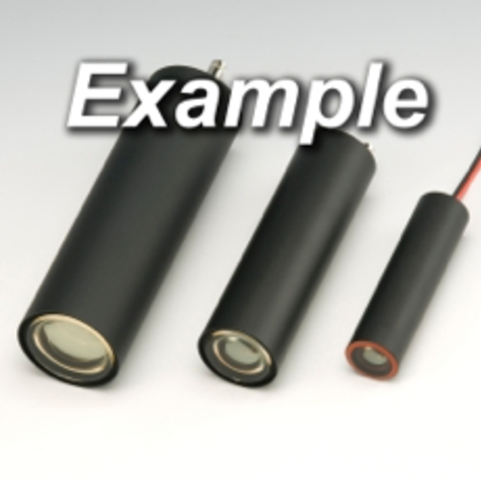
\includegraphics[scale=0.5]{./calorimetry/Pictures/fig5.pdf}
\caption{A picture of a PMT stolen from the web site of Hamamatsu corporation, one of the largest manufacturers of these devices.}
\label{fig:cal5}
\end{figure}

\;

\section{Sampling}

\noindent
Look at this picture of an EM shower in a sampling calorimeter.


\;
\;

\begin{figure}[h]
\centering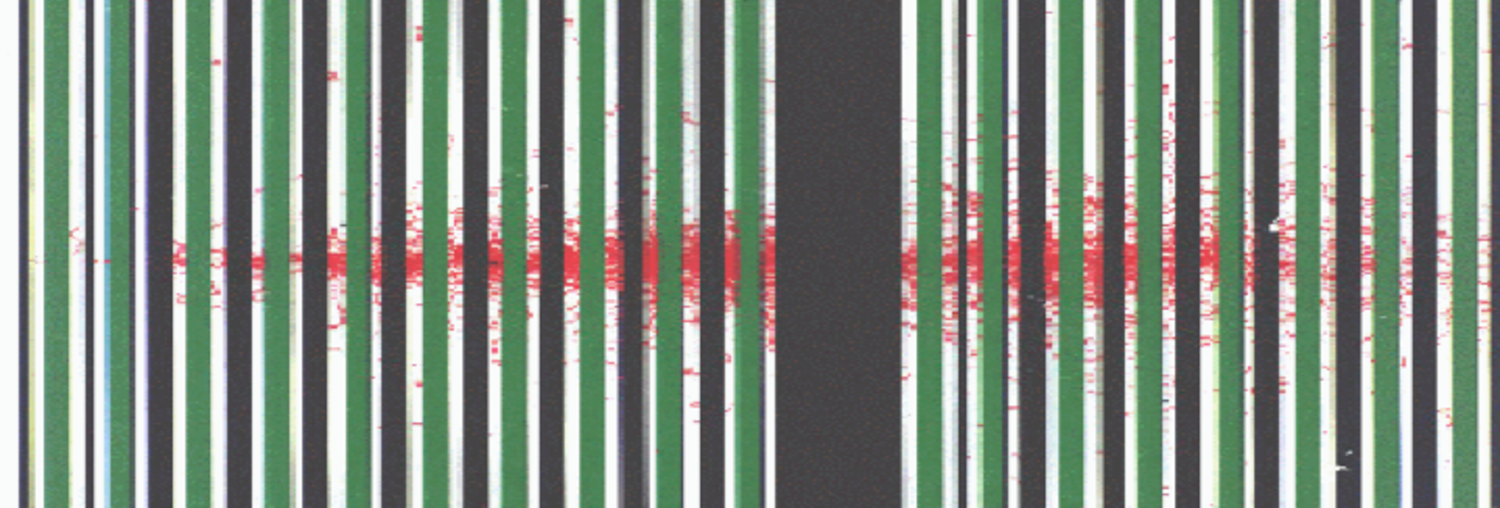
\includegraphics[scale=0.5]{./calorimetry/Pictures/fig6.pdf}
\caption{Schematic of an electromagnetic shower in a sampling calorimeter, as simulated by the GEANT4 shower simulation code. The colors denote various materials. The black denotes a high Z material, while the green denotes scintillator.}
\label{fig:cal6}
\end{figure}

\;

\noindent
The secondary particles only deposit some of their energy in the scintillator.  Most of it is deposited in the high Z material, which doesn$'$t produce light. Therefore, we are only measuring the energy of a small fraction of the shower, and thus a small fraction of the initial energy produced. We can correct for this on average:

\begin{equation}\hspace{34 mm}E_{estimated \: for \: initial\:  particle} = \frac{total \:amount\:  of\:  material \: in \: calorimeter}{amount \: of \: material\:  in \: plastic} E_{deposited \: in \: plastic}\end{equation}

\;
\;

\noindent
The ratio of the amounts of material is called the ``sampling fraction''. However, due to randomness in the shower process, sometimes a larger amount than this average will be deposited in the plastic, and sometimes less. This will lead to an uncertainty on the energy of the particle that started the shower. The smaller this ratio, the more accurate the measurement will be. For most calorimeters, though, the ratio is around 100.

\section{Energy Resolutions}

\noindent
How good is our calorimeter? This depends on how accurately it measures the energy of the initial particle. Sometimes, we take our calorimeters to test beams, and aim particles of known energy and momentum at them, to see how well they work. The figure below shows the result of aiming a beam of charged pions at the front face of the calorimeter.

\;
\;

\begin{figure}[h]
\centering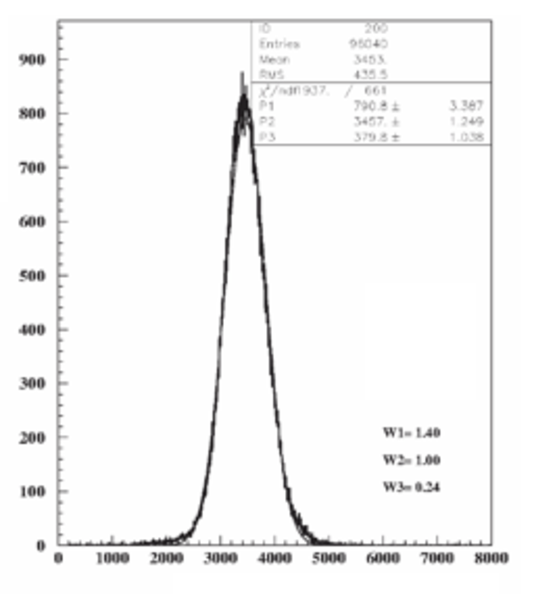
\includegraphics[scale=0.5]{./calorimetry/Pictures/fig7.pdf}
\caption{Charge collected from the detector when charged pions with a momentum of 300 GeV are steered into it.}
\label{fig:cal7}
\end{figure}

\;

\noindent
The output from the scintillator is charge, and so the x axis units are collected charge after amplification by the photomultiplier and other electronics. The detector is ``calibrated'' by setting the mean of this distribution (3457 fC) to the energy of the pions (300 GeV). The ratio of these numbers can be used to estimate the energy of the particle from the charge collected from the shower.  Of course, this is a very simplistic calibration. Getting an accurate calibration over a wide range of particle energies is a subject that could be a book in and of itself. 

\;
\noindent
As you can see, however, even though the incident particle always had the same energy, the amount of charge collected is not always the same. This is (mainly) because there are random fluctuations between the amount of energy deposited in the passive material and that deposited in the active material. The distribution of measured energies is well approximated by a Gaussian distribution:

\begin{equation}\hspace{20 mm}f(x,\mu,\sigma^{2}) = \frac{1}{\sigma\sqrt{2\pi }}\: e^{-(x-\mu)^{2}/2\sigma^{2}}\end{equation}

\;
\;

\noindent
The parameter $\mu$ is the mean of the distribution. The parameter $\sigma$ is the ``root mean square'' or ``sigma'' or the ``resolution''. It is a measure of the calorimeters ability to accurately measure the energy of the particle. In this figure, the mean is 3457 and sigma is 379.8. The fractional resolution is then the ratio of these two numbers, or 0.11.

\;
\noindent
The resolution for a calorimeter depends on the energy of the particle. The total number of secondary particles produced that cross the active material is proportional to the energy of the incident particle. The fluctuations on this number are proportional to the square root of this number, x. The fraction resolution (resolution/means) is thus proportional to $1/\sqrt{x}$.

\;
\noindent
There are other sources of resolution besides this, and so for a realistic calorimeter, the resolution is given by:

\begin{equation}\hspace{35 mm}\frac{\sigma }{E} = \frac{s}{\sqrt{E}} \oplus \frac{n}{E} \oplus C
\end{equation}

\;
\;

where s is called the ``sampling term'' and comes from the mechanism we discussed, n is called the ``noise term'' and is usually dominated by fluctuations in the measured charge due to electronics noise, and c is called the constant term, and is usually dominated by leakage of secondary particles out the back of the detector. The $\oplus$ symbol means ``add in quadrature''. To do this, square each term, add these squares, and take the square root.  As you learn more statistics, you will learn this is a common procedure when there is more than one source of randomness contributing to a measureable outcome.

\noindent The figure below shows the resolution versus energy for one of the CMS detector$'$s calorimeters.

\;
\;

\begin{figure}[h]
\centering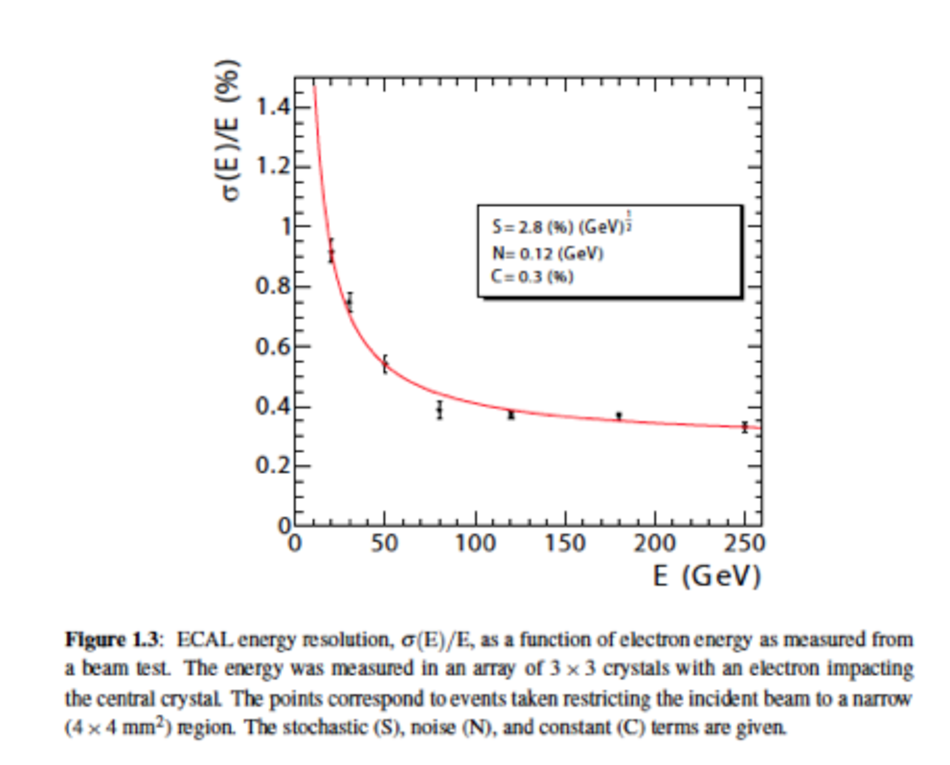
\includegraphics[scale=0.5]{./calorimetry/Pictures/fig9.pdf}
\caption{A figure stolen from JINST 3 S08004 showing the fractional resolution of the CMS barrel electromagnetic calorimeter as measured with electrons as a function of electron energy.}
\label{fig:cal8}
\end{figure}

\;

\section{read}

\;
$ \cdot \:$ Section 27.4 \url{http://pdg.lbl.gov/2011/reviews/rpp2011-rev-passage-particles-matter.pdf}

\;
\noindent
$ \cdot \:$  Section 28.9  \url{http://pdg.lbl.gov/2011/reviews/rpp2011-rev-particle-detectors-accel.pdf}

\;
\noindent
$ \cdot \:$  \url{http://journals.aps.org/rmp/abstract/10.1103/RevModPhys.75.1243}

\;
\noindent
$ \cdot \:$ \url{http://microcosm.web.cern.ch/microcosm/LHCGame/LHCGame.html}


\;
\noindent
$\cdot \:$ \url{http://www.sciencedirect.com/science/article/pii/S0168900211005572}

\;
\noindent
$\cdot \:$ \url{http://www.sciencedirect.com/science/article/pii/S0168900211019851}

\;
\noindent
$\cdot \:$ \url{http://www.sciencedirect.com/science/journal/01689002/666}

\;
\noindent
$\cdot \:$ \url{http://link.springer.com/article/10.1140$%$2Fepjc$%$2Fs10052-008-0573-yurl}

\;
\noindent
$\cdot \:$ \url{http://link.springer.com/article/10.1140$%$2Fepjc$%$2Fs10052-009-0959-5}

\;
\noindent
$\cdot \:$ \url{http://www.hamamatsu.com/resources/pdf/etd/PMT_handbook_v3aE.pdf}
